\documentclass[notheorems,aspectratio=169]{beamer}
\usepackage{algorithm2e}
\usepackage[T1]{fontenc}
\usepackage{lmodern}

\usepackage{cmap}
\usepackage[T2A]{fontenc}
\usepackage[utf8]{inputenc}
\usepackage{mathtext}
\usepackage[english,russian]{babel}
\usepackage{commath}
\usepackage{gensymb}
\usepackage{amsfonts}
\usepackage{amssymb}
\usepackage{amsmath}
\usepackage{amsthm}
\usepackage{mathtools}
\usepackage{indentfirst}
\usepackage{geometry}
\usepackage{tikz}
\usepackage{tkz-euclide}
\usetkzobj{all}
\usetikzlibrary{arrows,positioning}
\usetikzlibrary{shapes,snakes}
\usetikzlibrary{shapes.multipart}
\usepackage{graphicx}
\usepackage{epstopdf}
\usepackage{subcaption}
\usepackage{caption}
\usepackage{hyperref}
\usepackage{setspace}
\usepackage{float}
\usepackage{tcolorbox}
\usepackage{totcount}
\usepackage{xcntperchap}
\captionsetup{justification=centering}
\usepackage{pgfpages}
\usepackage{physics}
\usepackage{algorithm2e}

%\pgfpagesuselayout{4 on 1}[a4paper,border shrink=5mm, landscape]
\mode<presentation>
{
	\usetheme{Warsaw}
	\usecolortheme{whale}
	\setbeamercovered{transparent}
	\useoutertheme{infolines}
}

\regtotcounter{section}
\regtotcounter{subsection}
\RegisterCounters{section}{subsection}


\newtheorem{theorem}{Theorem}
\newtheorem{example}{Example}
\newtheorem{definition}{Definition}
\DeclarePairedDelimiter\ceil{\lceil}{\rceil}
\DeclarePairedDelimiter\floor{\lfloor}{\rfloor}
\DeclareUnicodeCharacter{2212}{-}
\setbeamercovered{invisible}
\setbeamertemplate{navigation symbols}{}
\usepackage{physics}

\addtobeamertemplate{frametitle}{\setlength{\parindent}{0em}}{}
\addtobeamertemplate{block begin}{\setlength{\parindent}{0em}}{\setlength{\parindent}{2em}}
\addtobeamertemplate{block example begin}{\setlength{\parindent}{0em}}{\setlength{\parindent}{2em}}

\makeatletter
\setbeamertemplate{footline}
{
	\leavevmode%
	\hbox{%
		\begin{beamercolorbox}[wd=.5\paperwidth,ht=2.25ex,dp=1ex,center]{title in head/foot}%
			\usebeamerfont{title in head/foot}\insertshorttitle
		\end{beamercolorbox}%
		\begin{beamercolorbox}[wd=.42\paperwidth,ht=2.25ex,dp=1ex,center]{author in head/foot}%
			\usebeamerfont{author in head/foot}\insertshortauthor\beamer@ifempty{\insertshortinstitute}{}{, \insertshortinstitute}
		\end{beamercolorbox}%
		\begin{beamercolorbox}[wd=0.07\paperwidth,ht=2.25ex,dp=1ex,right]{date in head/foot}%
			\insertframenumber{} / \inserttotalframenumber\hspace*{2ex} 
		\end{beamercolorbox}}%
	\vskip0pt%
}

\setbeamertemplate{itemize items}[circle]
\setbeamertemplate{enumerate items}[circle]

\DeclareMathOperator*{\argmax}{arg\,max}
\DeclareMathOperator*{\argmin}{arg\,min}


\makeatletter
\title{Тривиальные задачи геометрии -- выпуклая оболочка и пересечение выпуклых многогранников}
\author{Наталья Александровна Пономарева}
\institute[344 группа]{344 группа \\ Лаборатория распознавания изображений \\  СПбГУ}
\makeatletter
\subject{\@title}
\makeatother

\begin{document}
 
\begin{frame}
  \maketitle
  	\centering
  % \begin{tabular}[t]{rl}
	  % Руководитель: & Литвинов~Ю.\,В.\\
	  % Консультант: & Корчемкин~Д.\,А.\\
  % \end{tabular}
\end{frame}


\begin{frame}\frametitle{Выпуклая оболочка. Общие понятия и определения}
	\textbf{Выпуклой оболочкой} множества точек $X$ называется пересечение всех выпуклых множеств, 
	содержащих заданные точки, и обозначается $Conv(X)$.
	\begin{figure}
		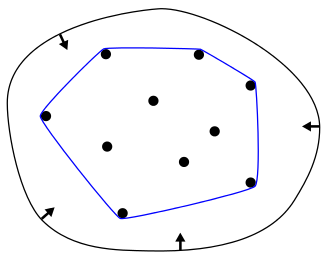
\includegraphics[height=0.5\textheight, keepaspectratio]{ConvexHull.png}
	\end{figure}
\end{frame}

\begin{frame}\frametitle{Выпуклая оболочка. Алгоритм Джарвиса}
	Самый простой подход -- ищем последовательно точки против часовой точки. 
	\begin{enumerate}
		\item Находим точку $p[0] = \underset{point \in X}{\operatorname{argmin(point.y)}} $. Если таких несколько, берём точку с наибольшей координатой $x$
		\item находим точку $p[1]$, как точку с наименьшим полярным углом относительно $p[0]$, как начала координат
		\item для последнего добавленного $p[i]$ ищем $p[i+1]$ среди всех недобавленных точек и $p[0]$ с максимальным углом между $p[i+1]p[i]$ и $p[i]p[i-1]$ (достаточно косинуса)
		\item если $p[i] == p[0]$ - алгоритм завершён
	\end{enumerate}
	\textbf{Время работы:} $O\left(nk \right)$
\end{frame}

\begin{frame}\frametitle{Выпуклая оболочка. Алгоритм Грэхэма}
	Пусть $p$ -- это стек, в котором хранятся текущие точки выпуклой оболочки, 
	$X$ -- исходное множество точек, $list$ -- упорядоченный список вершин.
	\begin{enumerate}
		\item Находим точку $p[0] = \underset{point \in X}{\operatorname{argmin(point.y)}} $. Если таких несколько, берём точку с наибольшей координатой $x$
		\item сортируем все остальные точки по полярному углу относительно $p[0]$ и записываем в $list$
		\item $p[1] := list[0]$ -- самая первая из отсортированных точек
		\item если $list.empty()$ - алгоритм завершён, осталось проверить условие из п.6 для $t = p[0]$
		\item иначе $t := list[j]$
		\item пока $t$ и две последних точки 
		в текущей оболочке $p[i]$ и $p[i - 1]$ образуют левый поворот, то есть 
		$|\left(p[i] - t\right) \times \left(p[i] - p[i - 1]\right)| > 0$, удаляем из оболочки pi
		\item добавляем в оболочку t
		\item переходим к пункту п.5, пока в списке есть точки
	\end{enumerate}
\end{frame}

\begin{frame}\frametitle{Выпуклая оболочка. Алгоритм Грэхэма. Доказательство}
	Докажем по индукции, что на каждом шаге $p$ является выпуклой оболочкой всех уже рассмотренных точек (или станет такой после проверки в пункте 6).
	\begin{itemize}
		\item База. Для двух первых точек утверждение, очевидно, выполняется.
		\item Индукционный переход. Пусть для $(i - 1)$ точки оболочка совпадет с $p[0]:p[i-1]$.
		1) Пусть $t_{i} \in Conv(X)$, то есть $t_{i}$ лежит в истинной выпуклой оболочке. 
		Тогда $Conv(X_{i-1} \cup t_{i}) = Conv(X_{i-1}) \cup t_{i} \backslash P$, где $P$ -- множество всех
		точек выпуклой оболочки, видимых из $t_{i}$. Так как для $(i-1)$ по индукционному предположению
		все совпадает, а $t_{i}$ положим в стек, то осталось показать, что $P$ совпадает с множеством точек,
		которые удалим из стека. 
	\end{itemize}
	Тогда по индукции оболочки совпадают и для $i = n$.
	
	\textbf{Время работы:} $O\left(n*\log(n)\right)$
\end{frame}

\begin{frame}\frametitle{Выпуклая оболочка. Алгоритм Чена}
	\begin{enumerate}
		\item Разобьём все множество на произвольные группы по $m$ штук в каждой, 
		тогда всего групп окажется $r = n / m$, $O\left(m * log(m)\right)$.
		\item для каждой группы запустим алгоритм Грэхэма, 
		\item начиная с самой нижней точки ищем выпуклую оболочку алгоритмом Джарвиса, но перебираем не все точки, а по одной из каждой группы (бинпоиском за  $O\left(\log(m)\right)$)
	\end{enumerate}
	\textbf{Время работы}: На втором шаге -- $O\left(r*m*\log(m)\right) = O\left(n*\log(m)\right)$. 
	На третьем шаге поиск по всем группам займёт $O\left(r*\log(m)\right)=O\left(\frac{n}{m}\log(m)\right)$. 
	Всего таких шагов будет k, значит общее время -- $O\left(\frac{k*n}{m}\log(m)\right)$. 
	Итоговое время -- $O\left(n\left(1+\frac{k}{m}\right)\log(m)\right)$. Минимум достигается при $m=k$, то есть $О\left(n*\log(k)\right)$.
\end{frame}

\begin{frame}\frametitle{Выпуклая оболочка. Алгоритм Чена}
	\textbf{Подбор кол-ва точек в выпуклой оболочке:} Положим $m = 2^{2^t}$. Начиная с маленьких m будем запускать наш алгоритм, причем если на некотором шаге Джарвис уже сделал m шагов, то мы выбрали наше m слишком маленьким, будем увеличивать, пока не станет $m \geq k$. Тогда общее время алгоритма -- 
	$ \sum_{t=1}^{\log\log k} O\left(n \log(2^{2^t})\right) = O(n) \sum_{t=1}^{\log\log k} O(2^t) \leq O\left(n \cdot 2^{1+O(\log\log k)}\right) = O(n \log k)$
\end{frame}

\begin{frame}\frametitle{Выпуклая оболочка в $R^n$.}
	\begin{itemize}
		\item Алгоритм QuickHull
		\item Алгоритм ``Заворачивание подарка``
	\end{itemize}
\end{frame}

\begin{frame}\frametitle{Проективное пространство. Общие понятия и определения}
	Пусть $V$ -- $(n+1)$-мерное векторное пространство.
	\textbf{$(n)$-мерным проективным пространством} называется пространство, состоящее из одномерных векторных подпространств в $V$, и обозначается $P_n$. 
	
	Зафиксируем в $V$ координаты $x_0, x_1,..., x_n$
	относительно какого-нибудь базиса $e_0, e_1,..., e_n$. Два ненулевых вектора
	$v = (x_0, x_1,..., x_n)$ и $w = (y_0, y_1,..., y_n)$
	задают одну и ту же точку $p \in P_n$, тогда и только тогда, когда их координаты пропорциональны. Это называется \textbf{однородные координаты}.
\end{frame}

\begin{frame}\frametitle{Проективное пространство. Преимущества}
	\begin{itemize}
		\item Точки на бесконечности
		\item Более простые формулы
		\item Двойственность: биекция между $[w,x,y]$ и $<w,x,y>$
	\end{itemize}
\end{frame}

\begin{frame}\frametitle{Пересечение полуплоскостей}
	Пересечение полуплоскостей может быть получено построением выпуклой оболочки в двойственном прострастве для множества точек, являющихся дуальным преобразованием исходных полуплоскостей
	\begin{figure}
		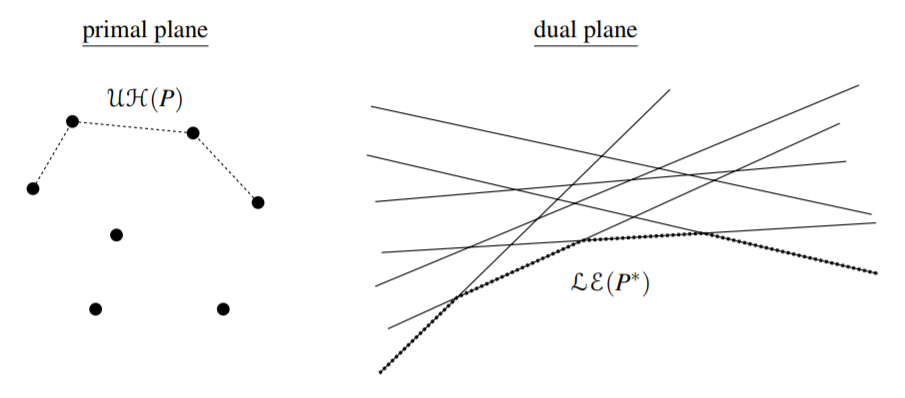
\includegraphics[height=0.5\textheight, keepaspectratio]{duality2.png}
	\end{figure}
\end{frame}

\begin{frame}\frametitle{Триангуляция Делоне. Общие понятия и определения}
	\textbf{Триангуляцией} называется планарный граф, все внутренние области которого являются треугольниками.
	
	\textbf{Триангуляцией Делоне} называется такое разбиение плоскости на
	треугольники с вершинами в заданных точках,
	что ни одна окружность, описанная вокруг любого из треугольников, не содержит других точек из разбиения.
	\begin{figure}
		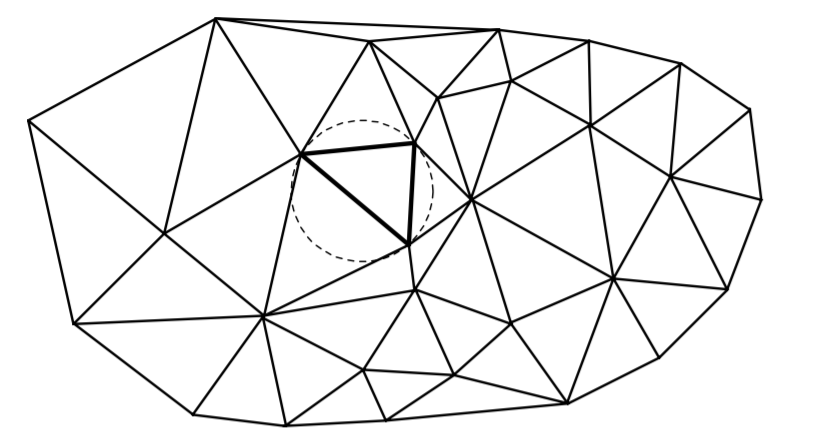
\includegraphics[height=0.5\textheight, keepaspectratio]{delone.png}
	\end{figure}
\end{frame}

\begin{frame}\frametitle{Триангуляция Делоне. Связь с выпуклой оболочкой}
	Рассмотрим параболоид $F = {(x,y,z): z = x^2+y^2}$. Возьмем некоторый набор
	точек и на плоскости и рассмотрим их отображения на параболоид. 
	Построим их выпуклую оболочку. Тогда проекции её нижних граней будут триангуляцией Делоне
	для начального набора точек. 
	\begin{figure}
		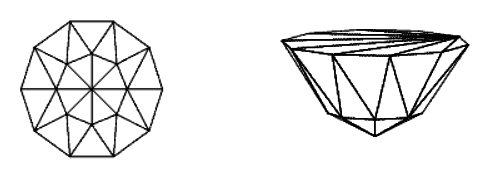
\includegraphics[height=0.5\textheight, keepaspectratio]{delone+obol.png}
	\end{figure}
\end{frame}

\begin{frame}\frametitle{Диаграмма Вороного. Общие понятия и определения}
	Для заданной точки $p_i \in X$
	\textbf{многоугольником Вороного} называется геометрическое место точек на плоскости,
	которые находятся к $p_i$ ближе, чем к любой другой точке $p_j \in X: j \neq i$. 
	
	\textbf{Диаграммой Вороного} заданного множества точек $X$ называется совокупность всех 
	многоугольников Вороного этих точек. 
	
	Если соединить все точки, соответствующие смежным ячейкам диаграммы Вороного,
	получится триангуляция Делоне для этого множества точек.
	\begin{figure}
		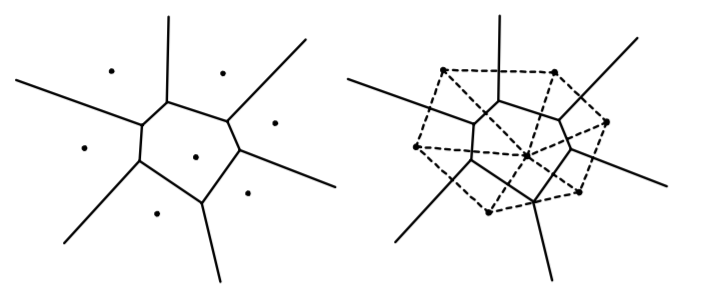
\includegraphics[height=0.5\textheight, keepaspectratio]{voronoj.png}
	\end{figure}
\end{frame}

\begin{frame}\frametitle{Условие Делоне}
	Триангуляцию Делоне можно получить из любой другой триангуляции по той же системе точек, 
	последовательно перестраивая пары соседних треугольников $ABC$ и $BCD$, не удовлетворяющих условию
	Делоне, в пары треугольников $ABD$ и $ACD$.
	\begin{figure}
		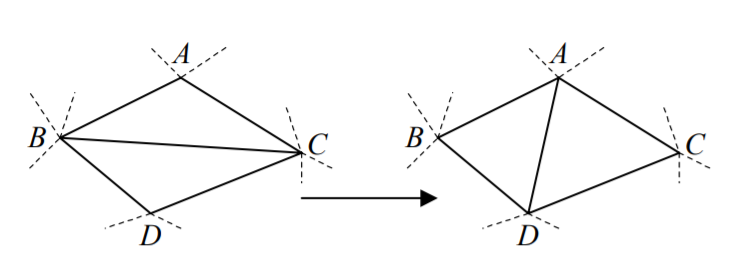
\includegraphics[height=0.5\textheight, keepaspectratio]{delone1.png}
	\end{figure}
\end{frame}

\begin{frame}\frametitle{Проверка условия Делоне}
	Через уравнение описанной окружности:
	$
	\begin{vmatrix}
	x^2+y^2& x& y& 1\\
	x_1^2+y_1^2& x_1& y_1& 1\\
	x_2^2+y_2^2& x_2& y_2& 1\\
	x_3^2+y_3^2& x_3& y_3& 1
	\end{vmatrix}
	= 0$
	
	\begin{itemize}
		\item предпосчитаем центры и радиусы окружностей заранее, тогда 
		$\forall (x_0, y_0): (x_0 - x_c)^2+(y_0-y_c)^2>r^2$
		\item достаточно считать только для половины треугольников, так как рассматриваем парами
	\end{itemize}
\end{frame}

\begin{frame}\frametitle{Проверка условия Делоне}
	Перепишем условие Делоне через углы:
	$$\forall (x_0, y_0): \angle p_1p_0p_3 + \angle p_1p_2p_3 \leq \pi
	\Leftrightarrow sin(\alpha+\beta) \geq 0 \Leftrightarrow 
	sin(\alpha)*cos(\beta)+cos(\alpha)*sin(\beta)\geq 0$$
	Синусы и косинусы можно выразить через скалярные и векторные произведения:
	$((x_0 - x_1)(y_0-y_3)-(x_0-x_3)(y_0-y_1))*
	((x_2 - x_1)(x_2-x_3)+(y_2-y_1)(y_2-y_3)) +$   
	$((x_0 - x_1)(x_0-x_3)+(y_0-y_3)(y_0-y_1))*
	((x_2 - x_1)(y_2-y_3)-(y_2-y_1)(x_2-x_3))\geq 0$
	\begin{figure}
		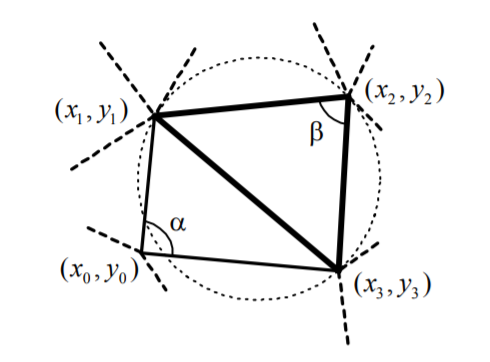
\includegraphics[height=0.3\textheight, keepaspectratio]{angles1.png}
	\end{figure}
\end{frame}


\begin{frame}\frametitle{Триангуляция Делоне. Алгоритм слияния ``Разделяй и властвуй``}
	\begin{itemize}
		\item Если $N = 3$, то построить триангуляцию из 1 треугольника,
		\item если $N = 4$, построить триангуляцию из 2 или 3 треугольников,
		\item если $N = 8$, разбить множество точек две части по 4 точки, рекурсивно применить алгоритм, а затем склеить триангуляции,
		\item если $N < 12$, разбить множество точек на
		две части по 3 и $(N − 3)$ точки, рекурсивно применить алгоритм, а затем
		склеить триангуляции,
		\item иначе разбить множество точек на две
		части по $\frac{N}{2}$ точек, рекурсивно применить алгоритм, а затем
		склеить триангуляции
	\end{itemize}
	\begin{figure}
		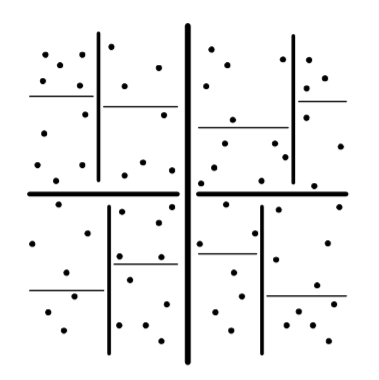
\includegraphics[height=0.2\textheight, keepaspectratio]{rv.png}
	\end{figure}
\end{frame}

\begin{frame}\frametitle{Триангуляция Делоне. Cлияние ``Удаляй и строй``}
	\begin{itemize}
		\item Построить 2 общие касательные, одна из которых называется ``базовой линией``,
		\item найти ближайший к базовой линии узел из обеих триангуляцией,
		\item построить треугольник на базовой линии и найденном узле, удалить все перекрываемые треугольники,
		\item новая базовая линия - одна из сторон треугольника,
		\item выполнять до достижения второй касательной.
	\end{itemize}
	\begin{figure}
		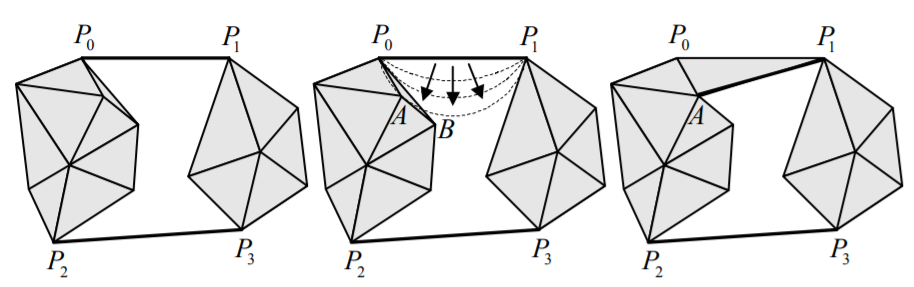
\includegraphics[height=0.4\textheight, keepaspectratio]{a.png}
	\end{figure}
\end{frame}

\begin{frame}\frametitle{Триангуляция Делоне. Cлияние ``Строй и перестраивай``}
	\begin{itemize}
		\item Построить 2 общие касательные, одна из которых называется ``базовой линией``,
		\item относительно текущей базовой линии рассматривают две следующие точки $N_1$ и $N_2$ вдоль границ
		сливаемых триангуляций,
		\item из двух возможных треугольников выбирают тот, который удовлетворяет условию Делоне, и тот, 
		у которого максимальный угол больше,
		\item новая базовая линия -- одна из сторон треугольника,
		\item выполнять до достижения второй касательной,
		\item проверить все построенные треугольники на выполнение условия Делоне с соседними и перестроить.
	\end{itemize}
	\begin{figure}
		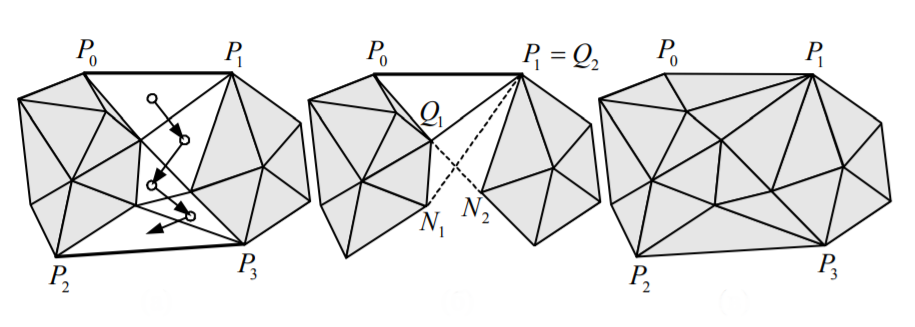
\includegraphics[height=0.3\textheight, keepaspectratio]{b.png}
	\end{figure}
\end{frame}

\begin{frame}\frametitle{Триангуляция Делоне. Cлияние ``Строй, перестраивая``}
	Аналогично предыдущему, только треугольники перестраиваем сразу. 
	При перестроении нужно изменять текущую базовую линию. 
	\begin{figure}
		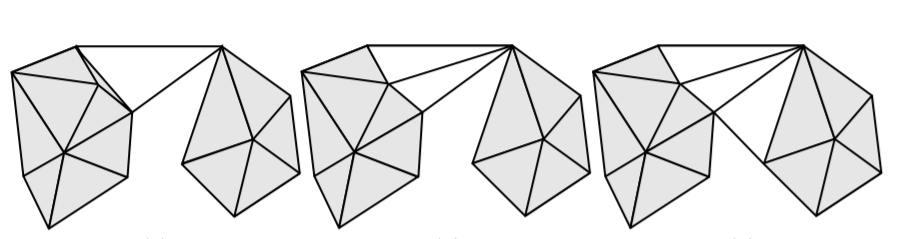
\includegraphics[height=0.5\textheight, keepaspectratio]{c.png}
	\end{figure}
	\textbf{Время работы}: Слияние за $O(N)$, слияний $\log(N)$ => $O(N\log(N))$
	
\end{frame}

\end{document}